%!TEX root = ../AST208-notes.tex

\section{The Difficulty with Direct Detection}

Suppose we want to observe exoplanets directly. Let's first estimate how far we have to look.  

\begin{exercisebox}[Mean distance to star in a sample]
\label{e.mean-distance}
The density of stars in the solar neighborhood is $\val{0.14}{\parsec^{-3}}$.  Suppose 50\% of the stars have planets, and we want a sample of about 20 planetary systems.  What would be the radius (in parsec) of the volume containing this many systems?  Given this radius, what is the average distance to a star in this sample?
\end{exercisebox}

Next let's estimate the difference in brightness between a planet and its host star. We shall use our solar system as an example.

\begin{exercisebox}[Ratio of flux from planet, star]
The Sun, which is at a distance of $\val{1}{\AU}$, has an apparent $V$-band magnitude $V_{\odot} = -26.74$.  At its closest approach of approximately $\val{4}{\AU}$, Jupiter has an apparent magnitude $V_{\jupiter} = -2.94$.  Compute the ratio of fluxes in $V$-band, i.e., $F_{\jupiter}/F_{\odot}$, if both Jupiter and the Sun were at the same distance.
\end{exercisebox}

Finally, we know that there is a limit to the angular resolution of a telescope. This limit is imposed by both the atmospheric seeing and the telescope optics.  Let's estimate how the angular separation of planet and star compares with a fiducial angular resolution.

\begin{exercisebox}[Resolving planets]
Jupiter's mean distance from the Sun is $\val{5.2}{\AU}$. Suppose we were to view the Sun-Jupiter system from the average distance derived in exercise \ref{e.mean-distance}; what would be the angular separation between Jupiter and the Sun?  How does this compare with the atmospheric seeing under good conditions?
\end{exercisebox}

As these exercises illustrate, imaging a planet directly is a daunting task. Astronomers have therefore resorted to indirect means, in which the host star is observed to vary due to the influence of the planet's gravitational force. This motivates a review of Kepler's problem.

\section{Planetary Orbits: Kepler}

Suppose we have a exoplanet system with a planet $p$ and a star $s$.  The vector from the star to the planet is $\rv_{sp} = \rv_{p}-\rv_{s}$, and the force that the star exerts on the planet is
\begin{equation}\label{e.newton}
	\bvec{F}_{sp} = -\frac{GM_{p}M_{s}}{|\rv_{sp}|^{3}} \rv_{sp}.
\end{equation}
The planet exerts a force on the star $\bvec{F}_{ps} = -\bvec{F}_{sp}$.

To make this problem more tractable, we shall put the origin of our coordinate system at the center of mass, as shown in Fig.~\ref{f.center-mass},
\begin{marginfigure}
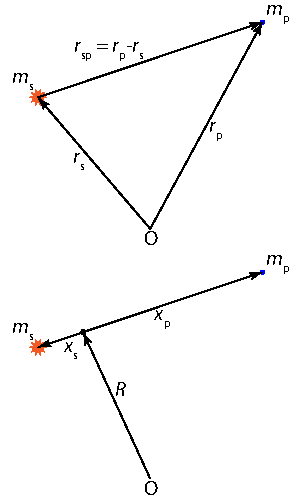
\includegraphics[width=\linewidth]{center-of-mass}
\caption[Center of mass]{Center of mass in a star-planet system.}
\label{f.center-mass}
\end{marginfigure}
\[ \bvec{R} = \frac{M_{s}\rv_{s} + M_{p}\rv_{p}}{M_{s}+M_{p}}; \]
in this frame the star and planet have positions 
\begin{eqnarray}
 \xv_{s} &=& \rv_{s}-\bvec{R} = -\frac{M_{p}}{M_{p}+M_{s}}\rv_{sp}\label{e.star-pos}\\
 \xv_{p} &=& \rv_{p}-\bvec{R} = \frac{M_{s}}{M_{p}+M_{s}}\rv_{sp}\label{e.planet-pos}
\end{eqnarray}
and hence accelerations
\begin{eqnarray*}
 \DDtt{\xv_{s}} &=& -\frac{M_{p}}{M_{p}+M_{s}}\DDtt{\rv_{sp}} \\
 \DDtt{\xv_{p}} &=& \frac{M_{s}}{M_{p}+M_{s}}\DDtt{\rv_{sp}}.
\end{eqnarray*}

If we substitute this acceleration into the equation of motion for the planet,
\[ M_{p}\DDtt{\xv_{p}} = \bvec{F}_{sp}, \]
and use eq.~(\ref{e.newton}) for $\bvec{F}_{sp}$, we get the reduced equation of motion
\begin{equation}\label{e.one-body}
 \DDtt{\rv_{sp}} = -G\frac{M_{s}+M_{p}}{|\rv_{sp}|^{3}} \rv_{sp}.
\end{equation}
We recover this same equation if we substitute the accelerations into the equation of motion for the star. Hence for a two body problem, we only need to solve equation~(\ref{e.one-body}) for $\rv_{sp}(t)$ and then use equations~(\ref{e.star-pos}) and (\ref{e.planet-pos}) to compute the positions $\xv_{s}(t),\xv_{p}(t)$ of the star and planet.

\begin{exercisebox}[Center-of mass for Sun-Jupiter]
Locate the center of mass for the Sun-Jupiter system:
\[ \frac{\Msun}{M_{\mathrm{\jupiter}}} = 1047; \qquad \rv_{\mathrm{\odot\jupiter}} = \val{5.2}{\AU}. \]
\end{exercisebox}

The solution to equation~(\ref{e.one-body}) is an elliptical orbit (Fig.~\ref{f.elliptical-orbit}) with the center-of-force at one focus of the ellipse.  The period $T$ depends on the semi-major axis $a$ of the ellipse,
\begin{equation}\label{e.period}
	T^{2} = \frac{4\pi^{2}}{G(M_{s}+M_{p})} a^{3}.
\end{equation}
Suppose the orbit is circular, so that $|\rv_{sp}|=a$ is constant.  Then by combining equations~(\ref{e.period}) and (\ref{e.star-pos}) we can find the orbital speed of the star,
\begin{equation}\label{e.star-velocity}
	v_{s} = \frac{M_{p}}{M_{s}+M_{p}} \times \frac{2\pi a}{T} = \left[\frac{GM_{p}}{a}
	\frac{M_{p}}{M_{s}+M_{p}}\right]^{1/2}.
\end{equation}
This speed is detectable via doppler shift of the stellar absorption lines.

\begin{marginfigure}
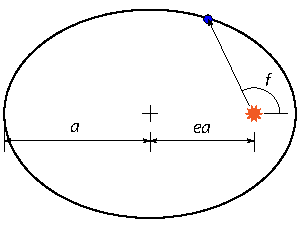
\includegraphics[width=\linewidth]{elliptical-orbit}
\caption[Orbital elements]{Orbital elements for a body moving in a gravitational potential about a fixed center of force, indicated by the yellow star.}
\label{f.elliptical-orbit}
\end{marginfigure}

\begin{exercisebox}[Orbital speed of the Sun]
\label{ex.sun-orbital-speed}
	Compute the orbital speed of the Sun for the two-body Sun-Jupiter system;
\[ \frac{\Msun}{M_{\mathrm{\jupiter}}} = 1047; \qquad \rv_{\mathrm{\odot\jupiter}} = \val{5.2}{\AU}. \]
\end{exercisebox}

\begin{exercisebox}[Doppler shift of Sun]
	What is the wavelength shift induced by the motion of the Sun, computed in exercise \ref{ex.sun-orbital-speed}, for an absorption line with rest wavelength $\val{600}{\nano\meter}$?
\end{exercisebox}

\section{Transits}

In \S~\ref{s.doppler} we derived the doppler shift for motion along our line-of-sight.
In general, however, the orbit is not edge-on, but rather inclined at an angle (Fig.~\ref{f.orbital-inclination}).
In this case the speed that is measured via doppler shift of stellar lines is $v_{s}\sin i$.  Thus, our problem becomes, given a measurement of period $T$ and projected speed $K = v_{s}\sin i$, what can we learn about the planet?

\begin{figure}[ht]
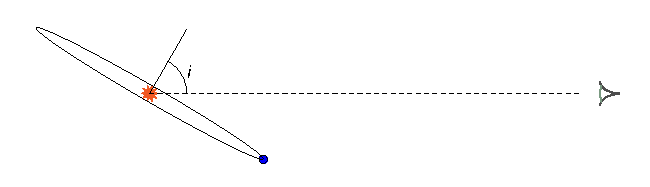
\includegraphics[width=\linewidth]{orbital-inclination}
\caption[Schematic of the inclination of a planetary orbit]{Schematic of the inclination of a planetary orbit to our line of sight.}
\label{f.orbital-inclination}
\end{figure}

We can combine equations~(\ref{e.period}) and (\ref{e.star-velocity}) into the form
\begin{equation}\label{e.mass-fcn}
	\frac{M_{p}^{3}\sin^{3}i}{(M_{s}+M_{p})^{2}} = \frac{K^{3}T}{2\pi G}.
\end{equation}
The right-hand side is in terms of the observed quantities $K$ and $T$, and is therefore determined from observations.  We expect $M_{s} \gg M_{p}$, and can usually estimate $M_{s}$ from spectroscopy of the star.  Even with this information, we can only determine $M_{p}\sin i$.

For systems with sufficiently large inclination, we will observe the planet to \emph{transit} the star, that is, to pass in front of the stellar disk. From Fig.~\ref{f.transit}, if
\begin{marginfigure}
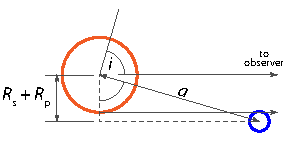
\includegraphics[width=\linewidth]{transit}
\caption[Schematic of a planetary transit]{Schematic of a planetary transit.}
\label{f.transit}
\end{marginfigure}
\[	\cos i < \frac{R_{s}+R_{p}}{a},	\]
then the light from the star will be partially blocked during some part of the orbit.\sidenote{We are assuming that the star is sufficiently far away that we can ignore the angle subtended by the star.}

\begin{exercisebox}[Inclination required to observe transit]
For the Sun-Jupiter system ($\Rsun = \val{\sci{6.96}{5}}{\kilo\meter}$, $R_{\jupiter}=\val{71\,400}{\kilo\meter}$, $a = \val{5.2}{\AU}$), what orbital inclination is required for an observer in a distant planetary system to witness a transit?
\end{exercisebox}

\newthought{What is the probability distribution of a star's inclination?}
To derive this, let's imagine each planet's orbital angular momentum as a vector having unit length.  We don't care about whether, from out perspective, the planet orbits counterclockwise or clockwise, so we put all of the arrows with $0\le i\le \pi/2$, as shown in figure~\ref{f.inclination-probability}.  

\begin{figure}[ht]
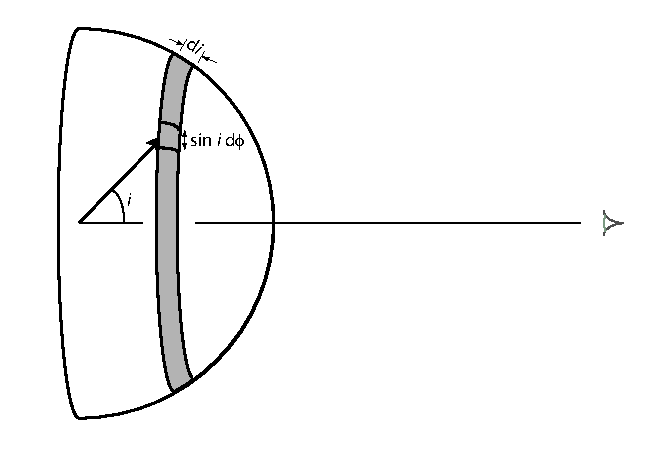
\includegraphics[width=\linewidth]{inclination-probability}
\caption[Schematic of the probability distribution of orbital inclination]{Schematic of the probability of the orbital inclination lying within $(i,i+\dif i)$ and $(\phi,\phi+\dif\phi)$.}
\label{f.inclination-probability}
\end{figure}

Now imagine a huge sample of planetary systems.  If the orbits are randomly distributed, then we expect the arrows to be evenly distributed over our hemisphere; as a result, the probability of a planet having inclination in $(i,i+\dif i)$ and azimuthal angle in $(\phi,\phi+\dif\phi)$ is the ratio of the area of that little coordinate patch to the area of the hemisphere,
\[ p(i,\phi)\,\dif i\,\dif \phi = \frac{\sin i\,\dif i\,\dif\phi}{2\pi}. \]
Since we aren't interested in the azimuthal angle, we can integrate over $\phi$ to find the probability distribution for a planet to have a given inclination, $p(i) = \sin i$.


\begin{exercisebox}[Mass-function and distribution of masses]
From a solar-mass star you measure a periodic doppler shift with $T = \val{3}{\yr}$ and $K = \val{18}{\meter\usk\second^{-1}}$.  What is the probability that the planet has a mass $>\val{2}{M_{\jupiter}}$? What is the probability that the planet has a mass $>\val{10}{M_{\jupiter}}$?
\end{exercisebox}

\begin{exercisebox}[Fraction of orbit in transit]
\begin{enumerate}\renewcommand{\labelenumi}{\alph{enumi})}
\item\label{e.transit-fraction}
For an edge-on, circular orbit, show that the fraction of the orbit during which the planet is in transit is
\[ f = \frac{T_{\mathrm{tr}}}{T} = \frac{R_{s}+R_{p}}{\pi a}, \]
where $a$ is the orbital separation.

\item\label{e.transit-duration}
Derive an expression for the transit duration $T_{\mathrm{tr}}$ in terms of $a$ and the masses and radii of the star and planet.

\item\label{e.transit-properties-jupiter}
For the Sun-Jupiter system, what is $f$ and $T_{\mathrm{tr}}$?

\end{enumerate}
\end{exercisebox}

